% 必要な項目ができた場合は適宜サブセクションを追加してください

%\include{begin}

% イベント名を記入する
\section{片付け(体育館)}
% 日時と場所を記入する
% 時刻は4桁で記入すること!
\subsection{日時・場所}
\begin{tabular}{p{2zw}rp{38zw}}
  日時 & : & 2019年4月6日(土) 11:55(イベントが終わり次第) $\sim$\\
  場所 & : & 体育館
\end{tabular}

% 目的を記入する
\subsection{目的}
先遣隊と後遣隊のメンバーが掃除する。来た時よりも美しく。

% イベントの概要やルールを記入する

% イベントのタイムスケジュールを記入する
% 時刻は必ず4桁(00:00)で記入すること!
% 時間の流れは途切れないように記述する!
\subsection{タイムスケジュール}
\begin{longtable}{p{3zw}p{39zw}}
  11:55 & \textbf{◎ 作業} \\
  		& \ \  \textbullet \ \ 昼食が終わり次第片付けを行う \\
        & \ \  \textbullet \ \ 小松,小島,西森は車を正面広間に移動する \\
        & \ \  \textbullet \ \ 横田は体育館,野田,以西は各研修室の持って帰る荷物とゴミを片付ける \\
        & \ \  \textbullet \ \ 片付けの際は宴用の余ったゴミ袋を使用。余らなかった場合は幡多の職員にゴミ袋をもらってくる \\
        & \ \  \textbullet \ \ 小松, 小島, 西森は車を移動したあと片付けに参加する \\
        & \ \  \textbullet \ \ 新入生が食堂からバスに移動するまでに机と椅子の片付けを行う \\\\
        
        & \ \  \textbullet \ \ 片付けが終了次第,食堂へ移動し昼食をとる \\\\
        
  
  13:10 & \textbf{◎ 昼食・幡多出発} \\
        & \ \  \textbullet \ \ 昼食を食べ終わり次第,片付け,忘れ物などをチェックする \\
        & \ \  \textbullet \ \ 全ての片付け終了後,幡多を出発する \\
\end{longtable}


% イベントに必要な役割と人数を記入する
% 担当者は決定次第追記する
% 記入例 ・司会者 2人(名前1、名前2)
\subsection{人員配置}
\begin{itemize}
\item 先遣隊:宮尾,小松,小島,横田,野田,以西
\item 後遣隊:西森,藤沢
\end{itemize}


% イベントを実施するときに新入生や先生、スタッフがどこに配置するかを記入する
% 図があるとわかりやすい
%\subsection{車の停車位置}
%\begin{figure}[h]
% \begin{center}
%  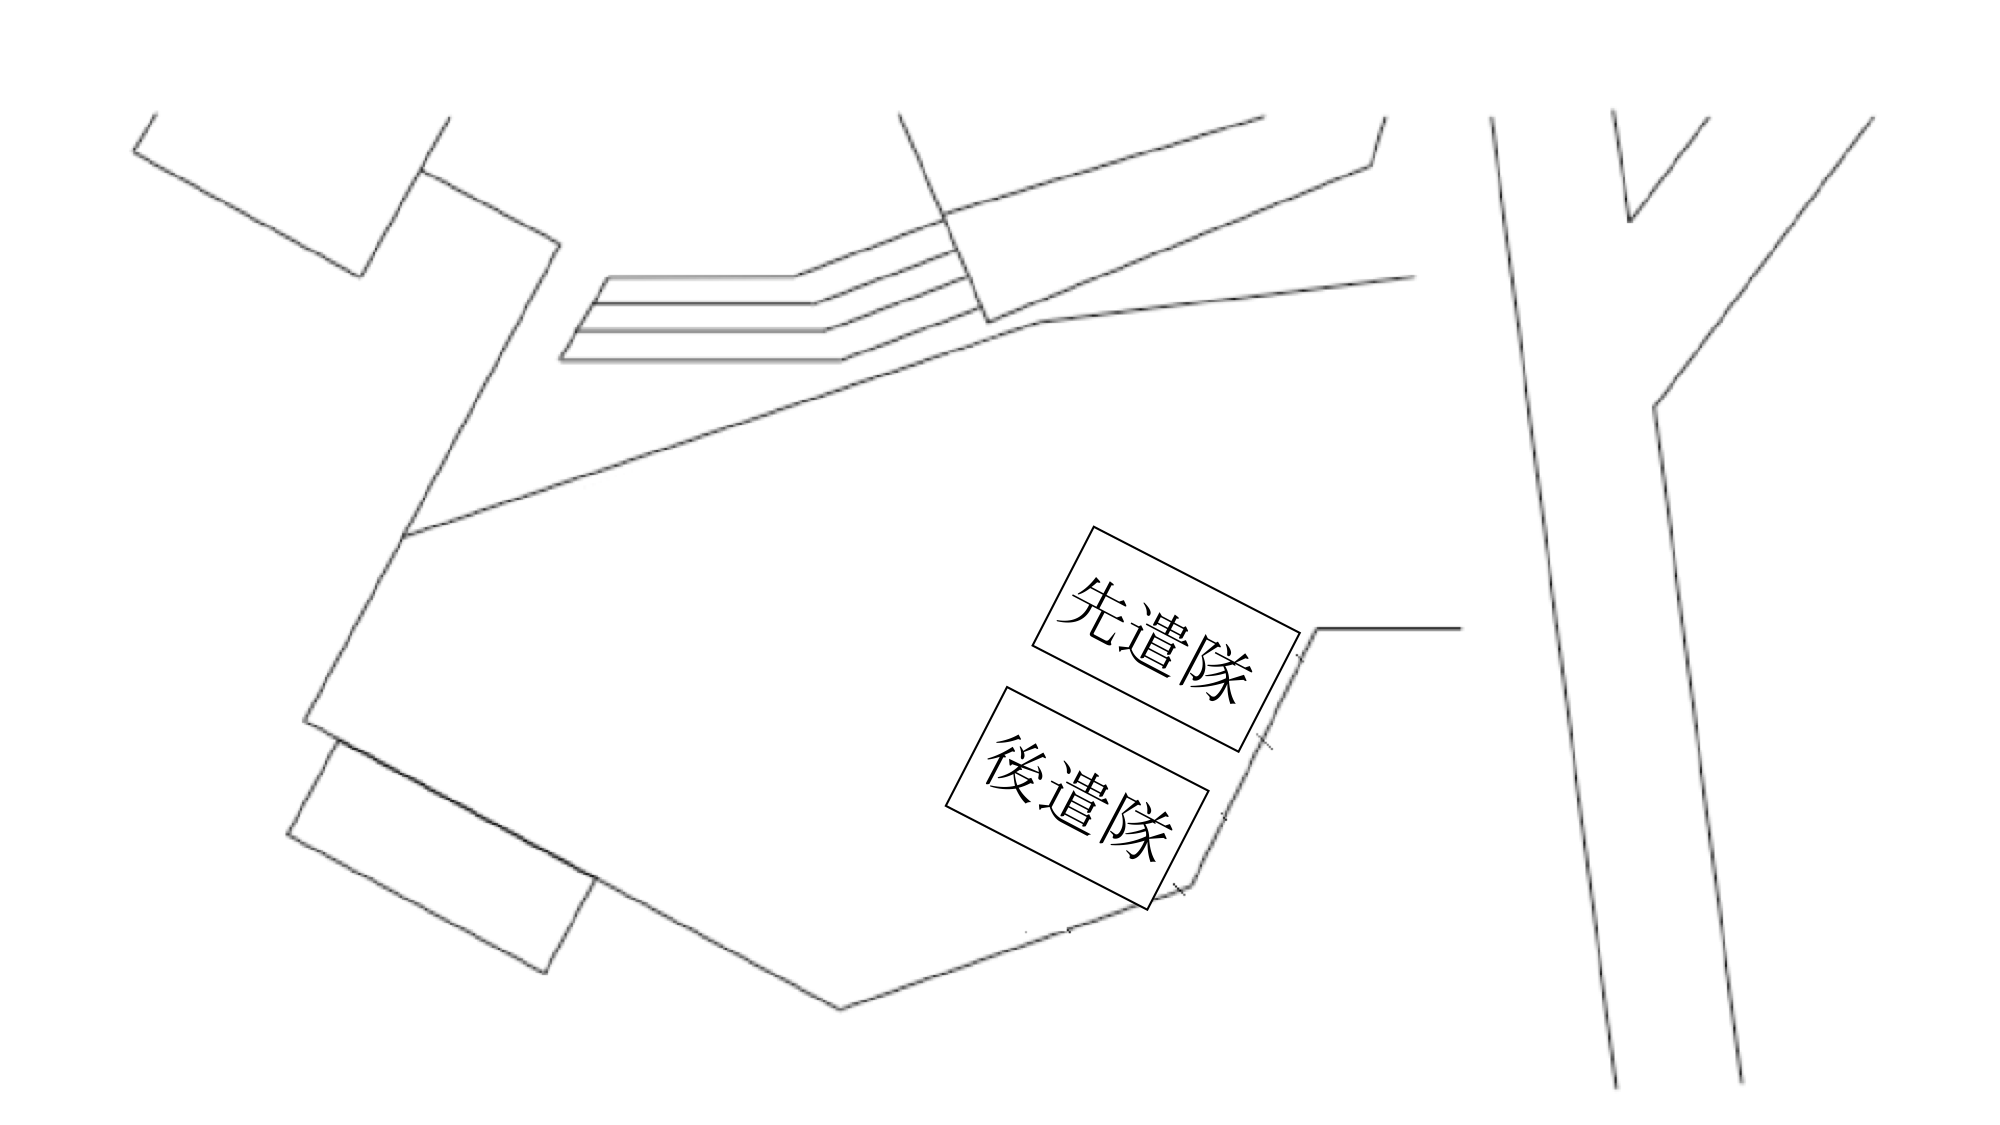
\includegraphics[width=115mm,height=70mm]{./27/syomenhiromacar.eps}
% \end{center}
% \caption{駐車場車配置}
%\end{figure}

\subsection{必要物品}
\begin{itemize}
\item 業務用ゴミ袋
\end{itemize}


\subsection{備考}
\begin{itemize}
\item ゴミは分別する
\item 机,椅子等の施設用具は幡多職員に片付ける場所を確認しておく
\item 忘れ物を入念にチェックする
\end{itemize}


%\include{end}

